%# -*- coding: utf-8-unix -*-
%%==================================================
%% impl.tex for SJTU Master Thesis
%%==================================================

%\bibliographystyle{sjtu2}%[此处用于每章都生产参考文献]
\chapter{系统需求分析与架构设计}
\label{chap:impl}

本章从需求角度和架构角度出发,介绍了Fornax在设计之初面临的功能性需求以及非功能性需求,并且基于这些需求,介绍了Fornax使用的架构,以及技术选型。

\section{需求分析}

持续集成与持续部署,已经成为了当下软件开发的最佳实践。因此也有越来越多的开发者希望能够在自己的开发流程中引入这样的实践来提高软件过程的效率与软件产品的质量。因此,持续集成与持续部署对于Fornax而言是非常重要的特性。持续集成要求Fornax必须与各种代码版本控制系统,比如Git,Svn等等进行交互。而持续部署要求Fornax要与应用的部署平台,也就是Kubernetes进行交互。

\begin{figure}[!htp]
  \centering
  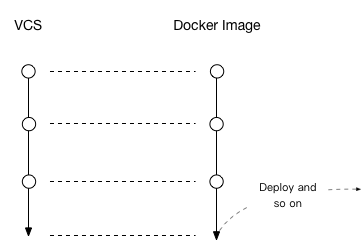
\includegraphics[width=0.5\textwidth]{impl/vcs.png}
  \bicaption[fig:vcs]{代码与镜像的版本控制}{代码与镜像的版本控制}{Fig}{}
\end{figure}

而除此之外,Fornax作为基于容器集群的版本管理与发布系统,与其他的持续集成与持续部署工具比较大的不同在于,Fornax还需要负责对于软件应用构建情况的版本管理。在传统的软件过程中,只有代码是被纳入版本控制的,运行时的环境,依赖,都没有版本控制的概念。这样的实践存在一些问题,比如在代码被回滚时,往往需要同时将运行时环境,包括依赖一起进行回滚,而在传统的做法中,这样往往需要重新打包依赖,过程耗时长而且自动化程度低。在引入了容器后,情况产生了一些变化。容器技术引入的镜像,可以很好地解决对于依赖和环境的版本管理问题。每当用户代码被构建完成后,可以将整个运行环境,依赖,和代码打包成一个镜像,这样当需要回滚时,只需要根据之前已经打包好的镜像重新启动一个新的容器即可。这使得软件的开发与部署有了新的实践方式,而这也是Fornax希望实现的。如图\ref{fig:vcs}所示,Fornax希望能够将代码的版本管理结合Docker镜像的版本管理,在每次代码产生变动时,都构建一个Docker镜像,并将其推送到Docker Registry中,当用户遇到需要回滚代码时,不需要再重新检出代码之后再次进行构建,而是通过Kubernetes集群的Rolling back的特性,直接将容器回滚到前一个版本的镜像。这样使得持续部署和应用回滚成为了更加简单的特性。除此之外,对于用户的构建日志,需要进行持久化地处理,以便用户之后便于排查问题,这也是Fornax需要解决的问题。

上述是Fornax的功能性需求,除此之外,Fornax还需要满足一些非功能性的需求,比如需要保持扩展性较强的设计,来满足以后可能遇到的新的需求。以及保证自身的无状态性,便于在需要时对Fornax进行水平扩容,采取多实例的方式来保证Fornax能够比较便捷地进行分布式地部署,提高系统的可用性。

\section{系统工作流}

在Fornax中,有两个比较重要的概念,一个是服务,一个是版本。这两个概念模型贯穿了整个Fornax的生命周期。服务,是引申自微服务概念中的服务,是指一个代码仓库对应的概念。一个服务拥有自己的版本控制系统类型,以及仓库的地址等信息。而版本则相对于服务而言要更加复杂一些,版本是指一次构建的版本,其中包含构建的版本的名字,描述,以及该版本在集群上的部署情况,比如部署在哪个集群的哪个节点上的信息之类。在Fornax的设计中,一个版本对应一个Docker镜像,当用户需要回滚版本时,只需要对已经部署的容器进行镜像的回滚即可。服务和版本的概念串联起了Fornax的工作流。

在Fornax中,如果要使用其提供的基于容器集群的版本管理与发布服务,需要先建立一个与传统的版本控制工具,如Git,Svn等的仓库概念对应的服务,在建立服务后,相关于该仓库的信息就会被Fornax记录,之后每当代码发生了变动,都会由Fornax来进行一次版本的构建,版本的构建环节中,Fornax并不是简单地把代码打包成为一个Docker的镜像,而是一个相对于传统的版本管理与发布工具而言要复杂一些的步骤。

在Fornax的设计中,所有有关在构建时的配置等信息,是记录在一个YAML格式的配置文件中的。因此Fornax在收到一个构建版本的请求时,会先确定在Clone下来的仓库中是否存在这样的配置文件,如果存在,就会根据配置文件中的配置来执行相关的步骤,否则就会如同其他的工具一样,直接进行镜像的构建和发布。以下讨论都建立在仓库中存在该配置文件的基础上而进行。

\begin{figure}[!htp]
  \centering
  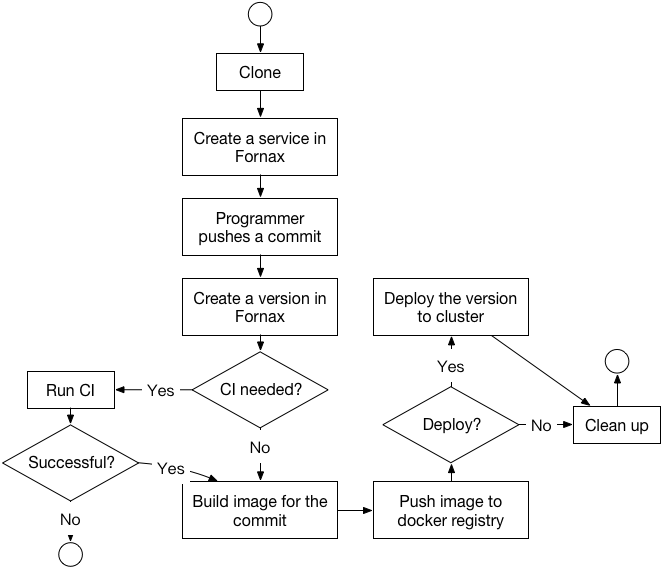
\includegraphics[width=0.7\textwidth]{impl/workflow.png}
  \bicaption[fig:workflow]{Fornax系统工作流}{Fornax系统工作流}{Fig}{}
\end{figure}

Fornax的工作流如图\ref{fig:workflow}所示,首先,Fornax会判断在配置文件中,是否有关于持续集成阶段的相关配置。如果存在这样的配置,Fornax会依据该配置文件,去进行相应的持续集成。通常持续集成的步骤会是执行持续集成测试,或者进行一些其他类型的测试以保证代码的质量,并根据持续集成的结果来判断是否需要打包新的版本。在Fornax中,持续集成的概念也是如此。在持续集成结束后,Fornax会根据结果来进行相应的操作,如果持续集成失败,那么整个流程都会结束,如果成功,Fornax会继续进行下一阶段的工作。值得一提的是,为了支持与现有的持续集成平台兼容,Fornax也允许使用Jenkins来进行持续集成,而不使用原本在Fornax中的持续集成,这样的妥协是为了保证能够尽快地接入现在主流的生产系统。

下一阶段的工作是构建和发布镜像。在这一阶段中,Fornax会在仓库中寻找目录下名为Dockerfile的文件,并根据该文件,去进行版本的构建。同时,为了满足一些自定义的需求,Fornax允许通过定义构建之前和之后的钩子(Hook)来执行一些用户定义的操作。在构建成镜像之后,Fornax会先将镜像存储在本地,在构建完成后,镜像会由Fornax推送到用户定义的Docker Registry或者推送到官方的Docker Registry上。

最后一阶段的工作是部署。在Fornax中,部署是指将打包好的镜像,在用户的集群中以容器的方式运行起来的过程,与持续集成相同,这也是自动化的过程。用户需要指定要部署的版本,选择集群,就可以将之前打包好的镜像发布到集群上。

在上述的阶段中,持续集成与持续部署是可选的阶段。而版本的构建会发布是每次代码发生变动时Fornax默认的行为。

\section{架构设计}

% 少了Daemon Manager

如图\ref{fig:design}所示,Fornax大致由八个模块构成。分别是API模块、异步事件管理模块、Docker管理模块、Docker后台管理模块、持续集成管理模块、版本管理系统管理模块、日志模块和数据库管理模块。这八个模块相互协同,实现了Fornax的所有功能。

\begin{figure}[!htp]
  \centering
  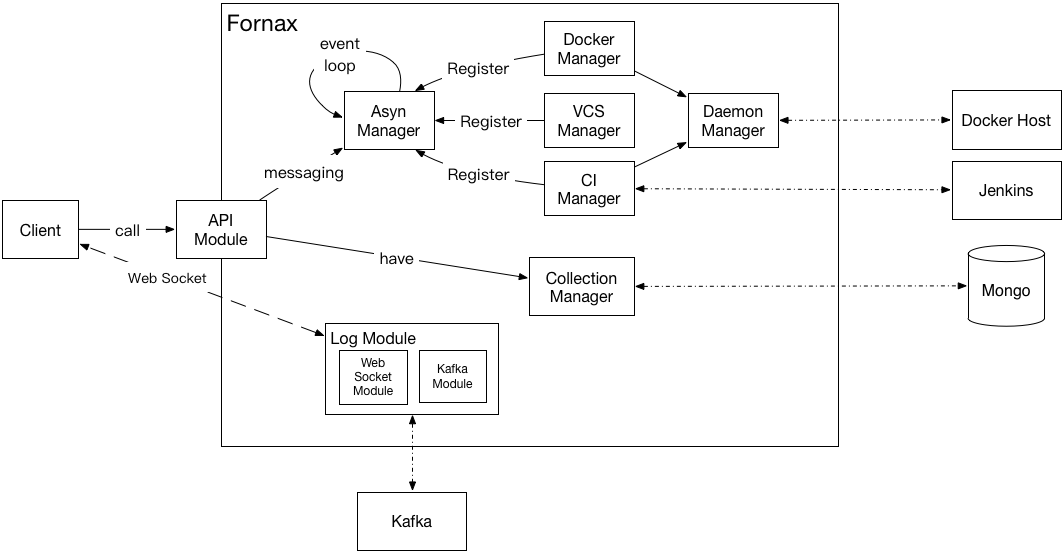
\includegraphics[width=0.9\textwidth]{impl/design.png}
  \bicaption[fig:design]{Fornax系统设计图}{Fornax系统设计图}{Fig}{}
\end{figure}

其中,API模块是将Fornax的服务以REST API的形式开放给客户端使用。这里的客户端不在Fornax的范畴内,可以是基于网页的客户端,或者是以命令行的方式来进行交互。API模块是整个Fornax系统对外交互的模块,它的职责在于接受来自客户端的请求,进行基本的认证与过滤,确保用户可信。之后,API模块会将过滤后的请求分发给相应的处理器进行处理。处理器也是API模块的一部分,他们会与异步事件管理模块交互,将请求交由其来进行调度与分配。

而异步事件管理模块,是其中比较重要的模块,也是实现难度比较大的模块。异步事件管理模块的职责是接受来自API模块发送过来的事件,然后将其加入到一个队列中,等待其被处理,并在处理后执行在API模块中定义的钩子函数,来进行自定义的收尾。异步事件管理器,是独立地运行在一个线程里的,不会阻塞主线程的运行,这也是异步操作带来的主要好处之一。目前Fornax中主要的两个事件是创建服务和创建版本,其他诸如查询服务内容,删除服务等等,因为处理起来比较快,不会过多地阻塞主线程,因此并没有进行异步化处理,而创建服务,涉及到对于代码仓库的Clone,创建版本,则不仅涉及该操作,还有持续集成任务的执行、镜像的构建、镜像的发布、容器的部署等一系列的事情,所以如果不以异步的方式去执行,会导致系统效率极低。因此Fornax对于这两种操作进行了异步的处理。

持续集成、版本管理、以及Docker构建镜像,都是在创建服务或者创建版本时需要使用的功能,所以三者对应的管理模块,会与异步事件管理模块交互,当一个事件在被处理时,异步事件管理模块会调用相应事件的处理器来进行处理,而三个模块就是在处理器中被其调用,进行相应的逻辑处理。

其中,版本管理系统管理模块负责与版本管理系统交互的功能实现。目前,版本管理系统管理模块包含Git,Svn对应的实现。当创建服务时,Fornax会将指定的代码仓库Clone下来,进行一些简单的校验。在创建版本时,为了防止代码仓库的污染,在每一步都会重新Clone代码仓库到Fornax指定的目录下。以及在发布镜像时,Fornax还会在发布的同时给构建镜像的提交打上一个标签,这同样需要版本管理系统管理模块支持。

Docker管理模块,是在构建和发布镜像时使用到的模块,Docker管理模块会与Docker Host进行交互,借由此来完成镜像的构建和发布。在目前的设计中,构建版本与服务时,对于Docker的依赖只限于构建镜像,和发布镜像,在持续集成环节中,还包括为每次持续集成构建隔离的网络环境等,这会在介绍持续集成管理模块时阐述。

Docker后台管理模块,是为了实现Fornax分布式的非功能性需求而实现的一个模块。在请求量比较大的时候,单个Docker Host必然没有办法满足Fornax的构建需要,因此引入了这样一个模块。该模块的职责是连接多个Docker Host进行构建,值得一提的是,该模块只有在定义了某些环境变量时才会被使用,默认情况下会使用一个Docker Host作为Docker的支持进行运行,这样设计是为了开发时的方便。

持续集成管理模块,是负责根据用户的仓库以及配置文件进行持续集成的模块。在Fornax中,持续集成是在容器内进行的。在一次持续集成中,Fornax会根据用户的配置,将用户自定义的持续集成以一个容器的方式运行起来。如果用户的代码存在运行时依赖,比如会依赖一个关系型数据库,Fornax也会支持通过容器方式先将用户在配置文件中定义好的依赖运行,再去运行用户自定义的持续集成的方式。依赖的容器和持续集成本身所在的容器通过自定义的网络环境相互连接,确保在一次持续集成任务中,容器间可以相互通信的同时,不会出现不同的持续集成任务之间容器可以相互沟通的问题,这是出于安全性的考量。持续集成管理模块,只有在存在配置文件,而且用户在配置文件中定义了相关持续集成阶段的配置时,才会被使用。

而日志模块,是相对独立的一个模块。它实现了一个基于WebSocket的协议,能够实时地将在各个阶段的日志推送给客户端。同时为了实现日志的持久化存储,引入了Kafka。具体实现的协议会在后文中进行更为详细的介绍。通过日志模块,用户可以在客户端看到每个阶段中所产生的日志。

最后,数据库模块,是对于数据库操作的封装。在API模块中,创建服务和版本都会向异步事件处理模块发送一个异步事件,而除此之外的所有操作,都只是单纯地通过对数据库的操作来完成。Fornax的数据库为MongoDB,是一个非关系型的数据库。因为服务与版本,都是非常灵活的模型。而为了满足这样的灵活性,非关系型数据库是比较好的选择,而MongoDB作为目前比较主流的生产可用的非关系型数据库,最终被采用。

上述八个模块,构成了Fornax。在第\ref{chap:detail}章中,会逐个介绍每个模块使用到的具体技术。
